\section{Software architecture views}
This section describes the software architecture views, it explains the subsystem decomposition, the hardware/software mapping, persistent data management and the concurrency.
\subsection{Subsystem decomposition}


\begin{figure}[h!]
  \centering
  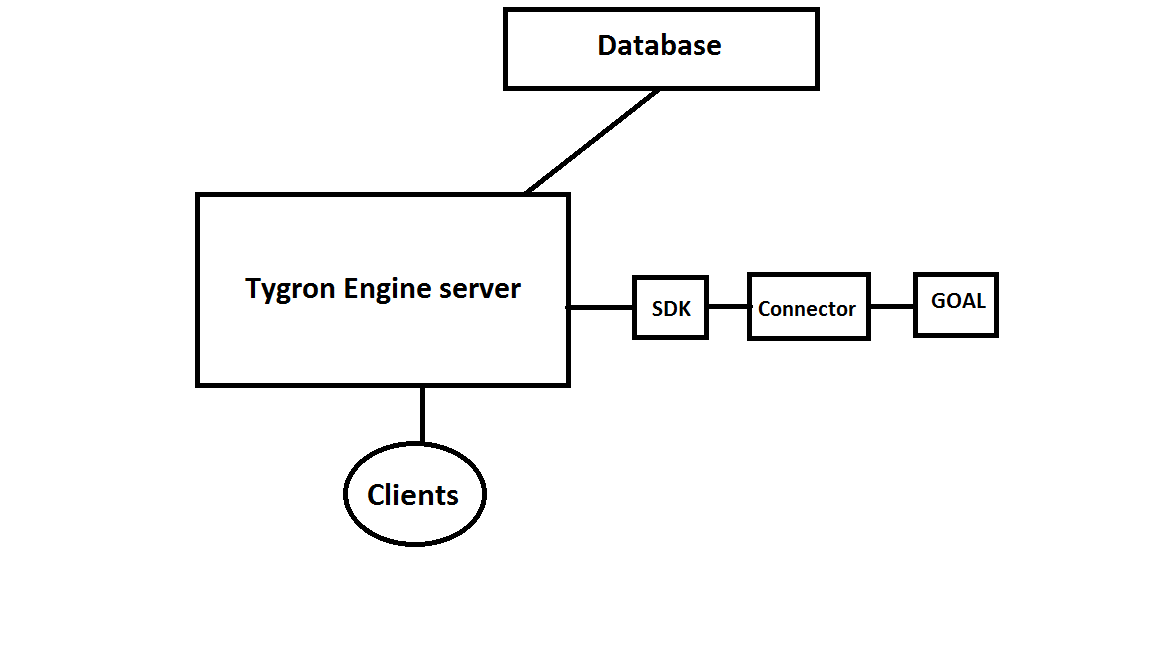
\includegraphics[scale=0.55]{Tygrondatabase3.png}
  \caption{Diagram of the Tygron Engine connected to the database and the GOAL agent.}
  \label{fig:tygron1}
\end{figure}
The architecture is divided into different subsystems. It consists of the database, Tygron engine server, several clients and several agents. In this section we will explain what each part is and does.

\begin{itemize}
	\item \textbf{The Database} \\ 
	The database in the system is used to save all kinds of data that is used to build the environment. This data contains for example the roads, buildings, rivers, etc.
	\item \textbf{The Tygron Engine Server (\textit{TES})} \\ 
	The Tygron Engine server is used to serve all the data to the correct clients and agents. The engine is an online 3D project software for urban planners, architects and engineers. It is a tool that streamlines the planning process and substantially reduces the time and costs involved in urban projects according to the Tygron website.
	\item \textbf{A Client} \\
	A client is a human interacting with the Tygron Engine Software. There can be multiple clients per \textit{TES}. The client can be a stakeholder and play the game according the strategy the stakeholder has in real live. 
	\item \textbf{The SDK} \\
	The SDK (Software Development Kit) is used to connect agents to the \textit{TES}.
	\item \textbf{An Agent} \\
	An agent is a computer controlled entity that acts like a client. There can be multiple agents per \textit{TES}. The agent can replace a client.
	\item \textbf{Connector} \\
	The connector is the link between the agent and the sdk. The agent needs the connector the run properly in the Tygron Engine. The connector generates the percepts for the agents and handles the actions that the agent performs. When an action change the environment, the agent can see the results of his action by looking at the percepts it receives from the connector.
\end{itemize}

\newpage
\subsection{Agent/Connector behaviour}
In this section some specific behaviour between the agent and the connector will be explained. The enhancements done to the connector will be explained and how they improve the development of an agent.

\subsubsection{Percepts}
In this section we'll describe some of the percepts in the connector and how are agent uses them.

\begin{itemize}
	\item \textbf{upgrade types} \\ 
	\begin{tabular}{ l l }
 		 Syntax & upgrade\_type($<$typeID$>$, $<$upgrade\_pair$>$) \\
  		Parameters &  $<$typeID$>$: Unique identifier for an upgrade type. 
				\\& $<$upgrade\_pair$>$: The pair of buildings of this upgrade. 
	\end{tabular}
	To enable us to upgrade a building the specific ID of that upgrade is needed. This ID is linked to a tuple that specifies the old building and the new building after the upgrade. When we receive this percept we can select the upgrade we need and then call the action to upgrade it. By adding this our agent can upgrade a building instead of demolish and rebuilding it.
	\item \textbf{Indicator} \\ 
	\begin{tabular}{ l l }
 		 Syntax & indicators($<$indID$>$, $<$currentValue$>$, $<$targetValue$>$) \\
  		Parameters &  $<$indID$>$: Unique identifier for an indicator. 
				\\& $<$currentValue$>$: The current value of the indicator. 
				\\& $<$targetvalue$>$: The target value of the indicator. 
	\end{tabular}
	The ultimate goal of the agent is to improve his score, he can do this by looking at its indicator scores and trying to improve these. To do this the agent needs to know what the score is and percept any changes. By enhancing the connector with this percept the agent is able to do this.
	\item \textbf{Indicator link} \\ 
	\begin{tabular}{ l l }
 		 Syntax & indicator\_link($<$indID$>$, $<$stakeIDs$>$, $<$name$>$, $<$weight$>$) \\
  		Parameters &  $<$indID$>$: Unique identifier for an indicator. 
				\\& $<$stakeIDs$>$: The ID of the stakeholder that has this indicator. 
				\\& $<$name$>$: The name of this indicator. 
				\\& $<$weight$>$: The weight that this indicator has for the total score. 
	\end{tabular}
	To enable our agent to see what the weights of a certain indicator are and which indicators are his an indicator link percept has been added to the connector. This percept helps to make the indicator percept more usefull for the agent.
	\item \textbf{Building} \\ 
	\begin{tabular}{ l l }
 		 Syntax & building($<$ID$>$, $<$name$>$, $<$categories$>$, $<$floors$>$, \\
		& $<$stakeholder\_ID$>$, $<$constructionYear$>$) \\
  		Parameters &  $<$ID$>$: Unique identifier for an indicator. 
				\\& $<$name$>$: The name of the building according to the tygron environment.
				\\& $<$categories$>$: The categorie of this building.
				\\& $<$floors$>$: The amount of floors of this building.
				\\& $<$stakeholder\_ID$>$: The ID of the stakeholder that owns this building.
				\\& $<$constructionYear$>$: The year the building was build.
	\end{tabular}
	The connector provides a building percept, that enables our agent to see which building he owns so that he can decide to for example destroy one of these buildings or upgrade it.

\end{itemize}

\newpage
\subsection{Hardware/software mapping}
In this section the hardware/software mapping Tygron uses will be explained, as well as the way our agent will be connected to this.

\subsubsection{Tygron}
Tygron has its own servers, from which it communicates with all other entities. For each group of users, there is a seperate server which contains the world that is used for the game and which this group of users can work on. The general Tygron server knows these other servers and will redirect the user to the particular server. So, when a customer wants to connect to Tygron, it will first connect to this general server. Also, this general server has contact with other servers which are not connected to Tygron. For example, when a customer wants to build a part of a city to play on, the general server will connect to some other servers that give information about this place, like where the buildings are and what the use of those buildings is. 

\subsubsection{Our project}
\begin{figure}[h!]
  \centering
  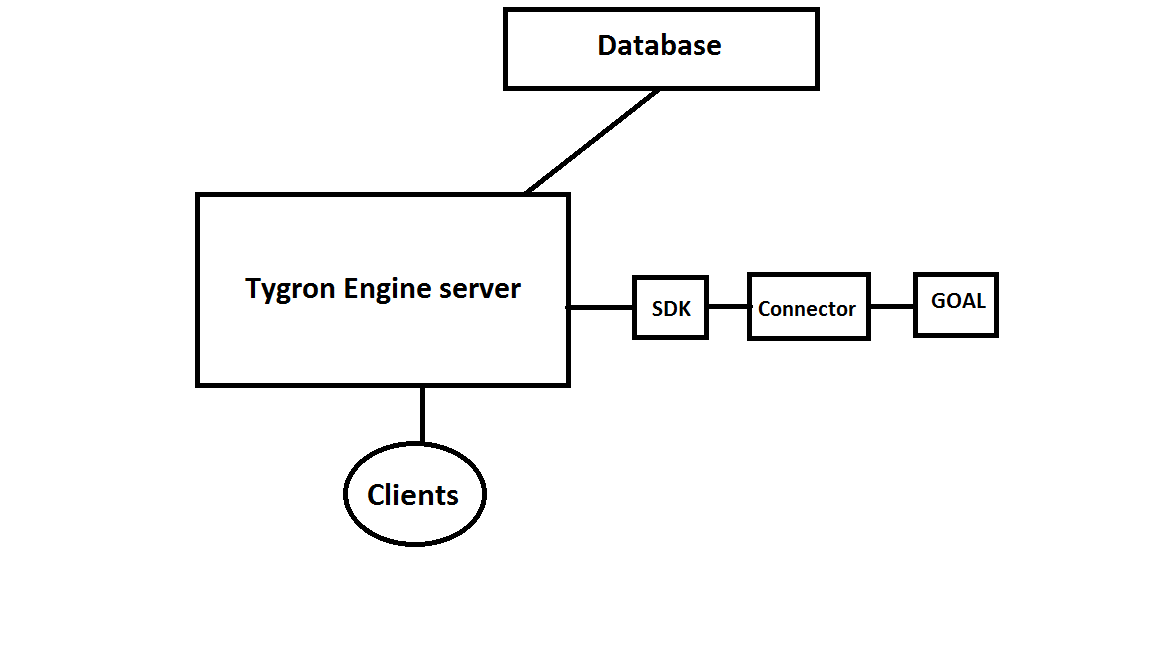
\includegraphics[scale=0.55]{Tygrondatabase3.png}
  \caption{Diagram of the Tygron Engine connected to the database and the GOAL agent.}
  \label{fig:tygron2}
\end{figure}
In this project there is an own server with all TU Delft students. But there is another thing that needs to be different: the way the connection is set up to that server. Since there are no humans, but agents to play the game, those agents need to connect in some way to the server. To do so, there is a connector between our instance and the server. This connector will use the goal code that is written by our group and will translate this into actions in the game. This way the agent can play the game. Figure 2 illustrates this.

\newpage
\subsection{Persistent data management}
The data management for our project envelops multiple parts. We have a part where the data for the game is stored and the data we need for running the agent. The first part is done by Tygron. When a new project is created it is stored in the Tygron database to which the clients can connect via the Tygron server. Any changes made in a session are then updated in the database, which are visible to all the other clients. Figure \ref{fig:tygron2} shows the diagram of the Tygron Engine connected to the database and the GOAL agent.

\begin{figure}[h!]
  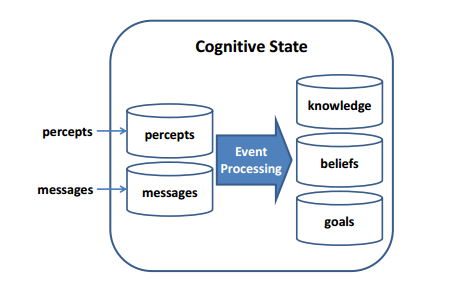
\includegraphics[width=\linewidth]{agentstate.png}
  \caption{Updating the agent's database.}
  \label{fig:agentstate1}
\end{figure}
In GOAL the data used by the agent is stored in multiple databases. The agent has a knowledge base which is the same for every environment that it might find itself in. This data is simply stored as GOAL code in the agent his GOAL files. The rest of the data that the agent uses is dynamic and its state is updated constantly according to the situation that the agent is currently in. Our agent maintains two different databases of facts. One database called the goal base consists of targets the agent wants to achieve. The other database is called the belief base and consists of facts that the agent believes are true (now). Figure \ref{fig:agentstate1} \cite{goal} shows how the databases of the agent are updated.



\newpage
\subsection{Concurrency}
Each group in the Virtual Humans for Serious Gaming context project will develop a cognitive agent, so there will be five roles and therefore multiple agents. An agent itself does not make use of concurrency, but all the agents together will run parallel and are running in one environment. When there are multiple agents running, there is concurrency. When we connect to an online server in the end, the overall system uses some networking, which also causes some concurrency. A crucial thing to find solutions for city design and development projects in a game is communication between the agents. The agents have to be able to communicate and find a solution together that fulfill the goals of the agents as much as possible.




